\usetikzlibrary{positioning, calc, shapes.multipart}
\resizebox{\textwidth}{!}{%
    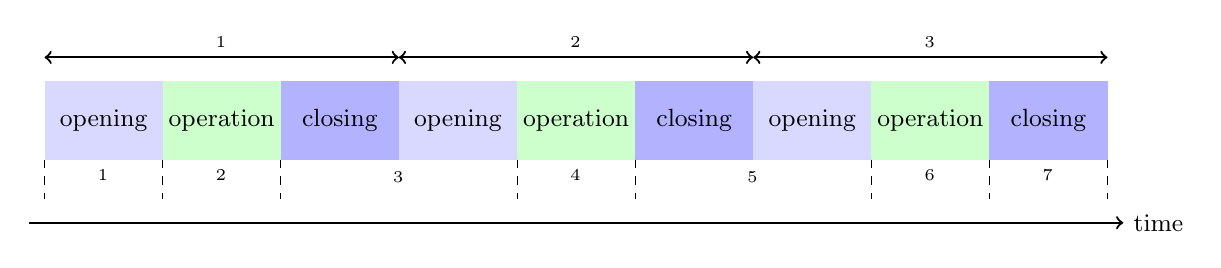
\begin{tikzpicture}[yscale=1, every node/.style={font=\small}]
        \def\w{1.5}  % phase width

        % Draw phases
        \path[fill=blue!15] (0,0) rectangle (\w,1);
        \node at (0.5*\w,0.5) {opening};

        \path[fill=green!20] (\w,0) rectangle (2*\w,1);
        \node at (1.5*\w,0.5) {operation};

        \path[fill=blue!30] (2*\w,0) rectangle (3*\w,1); % closing
        \path[fill=blue!15] (3*\w,0) rectangle (4*\w,1); % opening
        \node at (2.5*\w,0.5) {closing};
        \node at (3.5*\w,0.5) {opening};

        \path[fill=green!20] (4*\w,0) rectangle (5*\w,1);
        \node at (4.5*\w,0.5) {operation};

        \path[fill=blue!30] (5*\w,0) rectangle (6*\w,1); % closing
        \path[fill=blue!15] (6*\w,0) rectangle (7*\w,1); % opening
        \node at (5.5*\w,0.5) {closing};
        \node at (6.5*\w,0.5) {opening};

        \path[fill=green!20] (7*\w,0) rectangle (8*\w,1);
        \node at (7.5*\w,0.5) {operation};

        \path[fill=blue!30] (8*\w,0) rectangle (9*\w,1);
        \node at (8.5*\w,0.5) {closing};

        % Phase labels (only those outside closing+opening moved below)
        \node[anchor=north] at (0.5*\w,0) {$\phasePMPC_1$};
        \node[anchor=north] at (1.5*\w,0) {$\phasePMPC_2$};
        \node[anchor=north] at (4.5*\w,0) {$\phasePMPC_4$};
        \node[anchor=north] at (7.5*\w,0) {$\phasePMPC_6$};
        \node[anchor=north] at (8.5*\w,0) {$\phasePMPC_7$};

        % Custom placed labels for φ_3 and φ_5 under the refresh phase blocks
        \node at (3*\w, -0.22) {$\phasePMPC_3$};
        \node at (6*\w, -0.22) {$\phasePMPC_5$};

        % Stage brackets
        \draw[thick,<->] (0,1.3) -- (3*\w,1.3);
        \node[above] at (1.5*\w,1.3) {$\stagePMPC_1$};

        \draw[thick,<->] (3*\w,1.3) -- (6*\w,1.3);
        \node[above] at (4.5*\w,1.3) {$\stagePMPC_2$};

        \draw[thick,<->] (6*\w,1.3) -- (9*\w,1.3);
        \node[above] at (7.5*\w,1.3) {$\stagePMPC_3$};

        % Uniform dashed vertical lines
        \foreach \i in {0,1,2,4,5,7,8,9} {
            \draw[dashed, line width=0.3pt] (\i*\w,0) -- (\i*\w,-0.5);
        }

        % Time arrow
        \draw[->, thick] (-0.2, -0.8) -- ({9*\w + 0.2}, -0.8) node[right] {time};

    \end{tikzpicture}
}
